\section{Auswertung}
\subsection{Ersatzschaltbild Transformator}
\begin{enumerate}[label=\alph*)]
	\item Zeichnen Sie das vollständige einphasige Ersatzschaltbild (Sternschaltung) des
	      Transformators.
	      \begin{figure}[h!]
		      \begin{center}
			      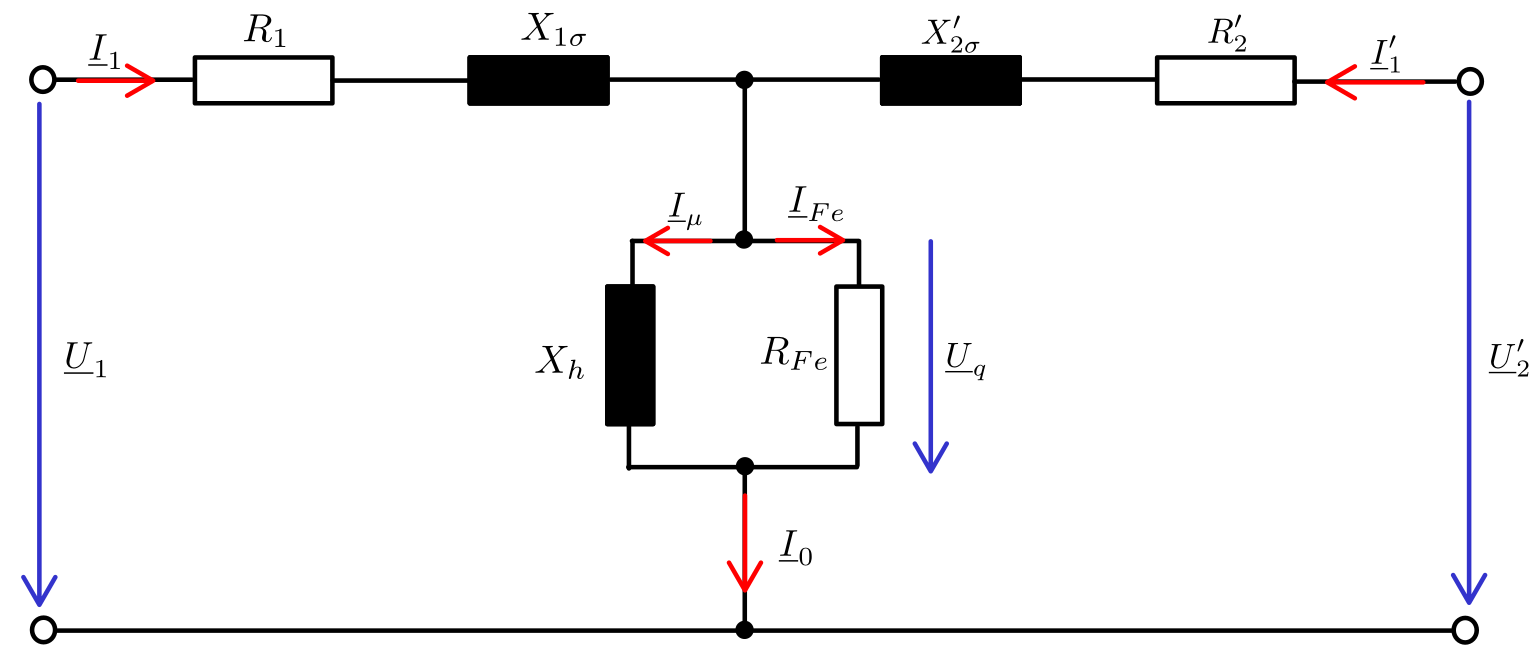
\includegraphics[width=0.95\textwidth]{img/4.1.1.1}
		      \end{center}
		      \caption{Vollständige einphasige ESP des Transformators}\label{img:2.1.1.1}
	      \end{figure}

	\item Bestimmen Sie die Leistung im Leerlauf auf der Primärseite nach Gleichung (16).
	      \begin{align*}
		      \underline S   & = \underline U_{12} \cdot \underline I_1^* + \underline U_{32}\cdot \underline I_3^* \\
		      \underline S   & = \underline U_{12} \cdot \underline I_1^* - \underline U_{23}\cdot \underline I_3^* \\
		      \underline S_0 & = 395\ V \cdot e^{j0^\circ} \cdot 0.45\ A \cdot e^{-(-j120^\circ)} -
		      393\ V \cdot e^{-j110^\circ}\cdot 0.45\ A \cdot e^{-(j25^\circ)}                                      \\
		      \underline S_0 & = 36,2\ W + j279\ \text{var} = 281\ VA\cdot e^{j82,6^\circ}                          \\
		      P_0            & = 36,2\ W                                                                            \\
		      Q_0            & = 279\ \text{var}
	      \end{align*}

	\item Bestimmen Sie die Wirkleistung im Kurzschlussfall auf der Sekundärseite nach
	      Gleichung (16). Gehen Sie dabei von einem symmetrischen System aus.
	      \begin{align*}
		      \underline S   & = \underline U_{12} \cdot \underline I_1^* + \underline U_{32}\cdot \underline I_3^* \\
		      \underline S   & = \underline U_{12} \cdot \underline I_1^* - \underline U_{23}\cdot \underline I_3^* \\
		      \underline S_K & = 12.5\ V \cdot e^{j0^\circ} \cdot 7,3\ A \cdot e^{-(-j52^\circ)}
		      - 12\ V \cdot e^{-j121^\circ}\cdot 7\ A \cdot e^{-(j65^\circ)}                                        \\
		      \underline S_K & = 140\ W+j 63\ \text{var} = 153\ VA \cdot e^{j24^\circ}                              \\
		      P_K            & = 140\ W                                                                             \\
		      Q_K            & = 63\ \text{var}
	      \end{align*}

	\item Ermitteln Sie die Daten des vollständigen Ersatzschaltbildes des Transformators
	      mit der Annahme $X_{1\sigma} = X'_{2\sigma} \text{ sowie } R_1 = R'_2$.
	      \begin{align*}
		      R_1                     & = R'_2                                                           \\
		      \Rightarrow R_1         & =\frac{P_{1K}}{2I_1^2}                                           \\
		      R_1                     & = \frac{140\ W}{3}\cdot \frac{1}{2(7,4\ A)^2}                    \\
		      R_1                     & = R'_2= 0,43\ \Omega                                             \\
		      X_{1\sigma}             & = X'_{2\sigma}                                                   \\
		      %
		      \Rightarrow X_{1\sigma} & =\frac{Q_{1K}}{2I_1^2}                                           \\
		      X_{1\sigma}             & = \frac{63\ \text{var}}{3}\cdot \frac{1}{2(7,4\ A)^2}            \\
		      X_{1\sigma}             & = X'_{2\sigma}= 0,19\ \Omega                                     \\
		      %
		      R_{FE}                  & = \frac{3\cdot(U_1)^2}{P_0}=\frac{3\cdot(U_{12})^2}{3 \cdot P_0}
		      = \frac{(U_{12})^2}{P_0}                                                                   \\
		      R_{FE}                  & = \frac{(395\ V)^2}{36,2\ W}                                     \\
		      R_{FE}                  & = 4,3\ k\Omega                                                   \\
		      %
		      X_{h}                   & = \frac{3\cdot(U_1)^2}{Q_0}=\frac{3\cdot(U_{12})^2}{3 \cdot Q_0}
		      = \frac{(U_{12})^2}{Q_0}                                                                   \\
		      X_{h}                   & = \frac{(395\ V)^2}{279\ \text{var}}                             \\
		      X_{h}                   & = 559,2\ k\Omega
	      \end{align*}

	\item Berechnen Sie anhand des Kurzschlussversuches die relative Kurzschlussspannung
	      des Transformators.
	      \begin{align*}
		      u_k & = \frac{U_K}{U_N}        \\
		      u_k & = \frac{12\ V}{400\ V}   \\
		      u_k & = 0,03\ \widehat{=}\ 3\%
	      \end{align*}

	      \pagebreak

\end{enumerate}

\subsection{Symmetrische Drehstromlast}
\begin{enumerate}[label=\alph*)]

	\item Berechnen Sie aus den Messwerten nach 3.2(b) die gemittelten Größen $U_m, I_m
		      \text{ und } \varphi_m$ (siehe Versuch E2-4), den Leistungsfaktor $\lambda =
		      \cos(\varphi_m)$, die Leistungen $S, P \text{ und } Q$ jeweils für die Primär-
	      und die Sekundärseite.

	      \textbf{Spannung}:\\\ \\
	      \begin{tcolorbox}[colback=gray!30,
			      colframe=black,
			      width=0.9\textwidth,
		      ]
		      \parbox{\textwidth}{

			      \begin{minipage}{0.5\textwidth}
				      \textbf{Primärseite:}\\ \ \\
				      \begin{align*}
					      U_{M.pri} & = \frac{U_{12} + U_{23} + U_{31}}{3} \\
					      U_{M.pri} & = \frac{378\ V + 371\ V + 372\ V}{3} \\
					      U_{M.pri} & = 373,67\ V
				      \end{align*}
			      \end{minipage}\hfill
			      \begin{minipage}{0.5\textwidth}
				      \textbf{Sekundärseite:}\\ \ \\
				      \begin{align*}
					      U_{M.sec} & = \frac{U_{12} + U_{23} + U_{31}}{3} \\
					      U_{M.sec} & = \frac{378\ V + 371\ V + 358\ V}{3} \\
					      U_{M.sec} & = 354\ V
				      \end{align*}
			      \end{minipage}
		      }
	      \end{tcolorbox}

	      \textbf{Strom}:\\\ \\
	      \begin{tcolorbox}[colback=gray!30,
			      colframe=black,
			      width=0.9\textwidth,
		      ]
		      \parbox{\textwidth}{

			      \begin{minipage}{0.5\textwidth}
				      \textbf{Primärseite:}\\ \ \\
				      \begin{align*}
					      I_{M.pri} & = \frac{I_{1} + I_{2} + I_{3}}{3} \\
					      I_{M.pri} & = \frac{7\ A + 7\ A + 7\ A}{3}    \\
					      I_{M.pri} & = 7\ A
				      \end{align*}
			      \end{minipage}\hfill
			      \begin{minipage}{0.5\textwidth}
				      \textbf{Sekundärseite:}\\ \ \\
				      \begin{align*}
					      I_{M.sec} & = \frac{I_{12} + I_{23} + I_{31}}{3} \\
					      I_{M.sec} & = \frac{7\ A + 7\ A + 6,7\ A}{3}     \\
					      I_{M.sec} & = 6,9\ A
				      \end{align*}
			      \end{minipage}
		      }
	      \end{tcolorbox}


	      \textbf{Phase}:\\\ \\
	      \begin{tcolorbox}[colback=gray!30,
			      colframe=black,
			      width=0.9\textwidth,
		      ]
		      \parbox{\textwidth}{

			      \begin{minipage}{0.5\textwidth}
				      \textbf{Primärseite:}\\ \ \\
				      \begin{align*}
					      \varphi_{M.pri} & = \frac{(\varphi_{1} + \varphi_{2} + \varphi_{3})-30^\circ}{3} \\
					      \varphi_{M.pri} & = \frac{65^\circ+68^\circ+67^\circ)-30^\circ}{3}               \\
					      \varphi_{M.pri} & = 36,7^\circ
				      \end{align*}
			      \end{minipage}\hfill
			      \begin{minipage}{0.5\textwidth}
				      \textbf{Sekundärseite:}\\ \ \\
				      \begin{align*}
					      \varphi_{M.sec} & = \frac{(\varphi_{1} + \varphi_{2} + \varphi_{3})-30^\circ}{3} \\
					      \varphi_{M.sec} & = \frac{64^\circ+65^\circ+63^\circ)-30^\circ}{3}               \\
					      \varphi_{M.sec} & = 34^\circ
				      \end{align*}
			      \end{minipage}
		      }
	      \end{tcolorbox}


	      \textbf{Scheinleistung:}\\ \ \\
	      \begin{tcolorbox}[colback=gray!30,
			      colframe=black,
			      width=0.9\textwidth,
		      ]
		      \parbox{\textwidth}{

			      \begin{minipage}{0.5\textwidth}
				      \textbf{Primärseite:}\\ \ \\
				      \begin{align*}
					      S_{pri} & = \sqrt3\cdot U_{M.pri}\cdot I_{M.pri} \\
					      S_{pri} & = \sqrt3\cdot 373,67\ V\cdot 7\ A      \\
					      S_{pri} & = 4,53\ \text{kVA}         \\
				      \end{align*}
			      \end{minipage}\hfill
			      \begin{minipage}{0.5\textwidth}
				      \textbf{Sekundärseite:}\\ \ \\
				      \begin{align*}
					      S_{sec} & = \sqrt3\cdot U_{M.sec}\cdot I_{M.sec} \\
					      S_{sec} & = \sqrt3\cdot 354\ V\cdot 6,9\ A       \\
					      S_{sec} & = 4,23\ \text{kVA}         \\
				      \end{align*}
			      \end{minipage}
		      }
	      \end{tcolorbox}


	      \pagebreak
	      \textbf{Wirkleistung:}\\ \ \\
	      \begin{tcolorbox}[colback=gray!30,
			      colframe=black,
			      width=0.9\textwidth,
		      ]
		      \parbox{\textwidth}{

			      \begin{minipage}{0.5\textwidth}
				      \textbf{Primärseite:}\\ \ \\
				      \begin{align*}
					      P_{pri} & = S_{pri} \cdot \cos(\varphi_{M.pri})      \\
					      P_{pri} & = 4,53\ \text{kVA} \cdot \cos(36,67^\circ) \\
					      P_{pri} & = 3,63\ kW
				      \end{align*}
			      \end{minipage}\hfill
			      \begin{minipage}{0.5\textwidth}
				      \textbf{Sekundärseite:}\\ \ \\
				      \begin{align*}
					      P_{sec} & = S_{sec} \cdot \cos(\varphi_{M.sec})   \\
					      P_{sec} & = 4,23\ \text{kVA} \cdot \cos(34^\circ) \\
					      P_{sec} & = 3,51\ kW
				      \end{align*}
			      \end{minipage}
		      }
	      \end{tcolorbox}

	      \textbf{Blindleistung}\\ \ \\
	      \begin{tcolorbox}[colback=gray!30,
			      colframe=black,
			      width=0.9\textwidth,
		      ]
		      \parbox{\textwidth}{

			      \begin{minipage}{0.5\textwidth}
				      \textbf{Primärseite:}\\ \ \\
				      \begin{align*}
					      Q_{pri} & = S_{pri} \cdot \sin(\varphi_{M.pri})      \\
					      P_{pri} & = 4,53\ \text{kVA} \cdot \sin(36,67^\circ) \\
					      Q_{pri} & = 2,71\ \text{var}
				      \end{align*}
			      \end{minipage}\hfill
			      \begin{minipage}{0.5\textwidth}
				      \textbf{Sekundärseite:}\\ \ \\
				      \begin{align*}
					      Q_{sec} & = S_{sec} \cdot \sin(\varphi_{M.sec})   \\
					      P_{sec} & = 4,23\ \text{kVA} \cdot \sin(34^\circ) \\
					      Q_{sec} & = 2,37\ \text{var}
				      \end{align*}
			      \end{minipage}
		      }
	      \end{tcolorbox}

	      \textbf{Leistungsfaktor}\\ \ \\
	      \begin{tcolorbox}[colback=gray!30,
			      colframe=black,
			      width=0.9\textwidth,
		      ]
		      \parbox{\textwidth}{

			      \begin{minipage}{0.5\textwidth}
				      \textbf{Primärseite:}\\ \ \\
				      \begin{align*}
					      \lambda_{pri} & = \cos{(\varphi)}   \\
					      \lambda_{pri} & = \cos (36,7^\circ) \\
					      \lambda_{pri} & = 0,8
				      \end{align*}
			      \end{minipage}\hfill
			      \begin{minipage}{0.5\textwidth}
				      \textbf{Sekundärseite:}\\ \ \\
				      \begin{align*}
					      \lambda_{sec} & = \cos{(\varphi)} \\
					      \lambda_{sec} & = \cos (34^\circ) \\
					      \lambda_{sec} & = 0,83
				      \end{align*}
			      \end{minipage}
		      }
	      \end{tcolorbox}

	      \ \\
	\item Berechnen Sie die Verlustleistung des Transformators sowie den Wirkungsgrad mit
	      den Ergebnissen aus 4.2(a).

	      \begin{minipage}[r]{0.5\linewidth}
		      \begin{align*}
			      S_{V} & = S_{pri} - S_{sec}       \\
			      S_{V} & = (4,53 - 4,23)\ \text{kVA} \\
			      S_{V} & = 300\ VA                 \\
			      P_{V} & = P_{pri} - P_{sec}       \\
			      P_{V} & = (3,63 - 3,51)\ kW          \\
			      P_{V} & = 120\ W                   \\
			      Q_{V} & = Q_{pri} - Q_{sec}       \\
			      Q_{V} & = (2,71 - 2,27)\ \text{var} \\
			      Q_{V} & = 340\ \text{var}
		      \end{align*}
	      \end{minipage}
	      \begin{minipage}[l]{0.5\linewidth}
		      \begin{align*}
			      \eta_S & = \frac{S_{sec}}{S_{pri}} \\
			      \eta_S & = 0,93\ \widehat{=}\ 93\% \\
			      \eta_P & = \frac{P_{sec}}{P_{pri}} \\
			      \eta_P & = 0,97\ \widehat{=}\ 97\% \\
			      \eta_Q & = \frac{Q_{sec}}{Q_{pri}} \\
			      \eta_P & = 0,88\ \widehat{=}\ 88\% \\
		      \end{align*}
	      \end{minipage}
	      \pagebreak

	\item Bestimmen Sie die Verlustleistung für 3.2(b) nach 2.1(d) und vergleichen Sie
	      das Ergebnis mit dem Wert aus 4.2(b). Begründen Sie Ihre Beobachtungen.\\
	      \begin{minipage}[r]{0.5\linewidth}
		      \begin{align*}
			      P_{FE} & = P_0\ \left(\frac{U}{U_N}\right)^2              \\
			      P_{FE} & = -43,1\ W\ \left(\frac{373\ V}{400\ V}\right)^2 \\
			      P_{FE} & = -37,477\ W
			      \\
			      P_{Cu} & = P_K\ \left(\frac{I}{I_N}\right)^2              \\
			      P_{Cu} & = 113\ W\ \left(\frac{7\ A}{7,2\ A}\right)^2     \\
			      P_{Cu} & = 106,909\ W
		      \end{align*}
	      \end{minipage}
	      \begin{minipage}[l]{0.5\linewidth}
		      \begin{align*}
			      P_{V} & = P_{FE} \ +\ P_{Cu}                                  \\
			      P_{V} & = -37,477\ W + 106,909\ W                             \\
			      P_{V} & = 69,33\ W
			      \\
			      \eta  & = 1-\frac{P_{v}}{S}                                   \\
			      \eta  & = 1- \frac{69,33\ W}{\sqrt{3}\cdot 354\ V\cdot 7\ A } \\
			      \eta  & = 0,9838
		      \end{align*}
	      \end{minipage}

	\item Berechnen Sie aus den Messwerten nach 3.2(b) und dem Übersetzungsverhältnis ü
	      den relativen Spannungsfall $\Delta u'_2$!\\ \ \\

	      \begin{minipage}[r]{0.5\linewidth}
		      \begin{align*}
			      U_1 & = ü\cdot U_2            \\
			      ü   & = \frac{U_1}{U_2}       \\
			      ü   & = \frac{373\ V}{354\ V} \\
			      ü   & = 1,053                 \\
			      ü   & \approx 1
		      \end{align*}
	      \end{minipage}
	      \begin{minipage}[l]{0.5\linewidth}
		      \begin{align*}
			      I_2 & = ü\cdot I_1          \\
			      ü   & = \frac{I_2}{I_1}     \\
			      ü   & = \frac{6,9\ A}{7\ A} \\
			      ü   & = 0,985               \\
			      ü   & \approx 1
		      \end{align*}
	      \end{minipage}

	\item Bestimmen Sie anhand der Formeln (11) - (13) den relativen Spannungsabfall für
	      3.2(b).

	      \begin{align*}
		      \Delta u'_2 & = \frac{U_1\ -\ U'_2}{U_1}                       \\
		      \Delta u'_2 & = \frac{373\ V -\frac{373\ V}{\sqrt{3}}}{373\ V} \\
		      \Delta u'_2 & = 0,422                                          \\
	      \end{align*}
	      \begin{align*}
		      U_l         & = I_1(R_K\cos(\varphi_2)+X_K\sin(\varphi_2))                              \\
		      U_l         & = 7\ A\ (33,7\ \Omega\ \cos(-46^\circ)\ +\ 40,1\ \Omega\ \sin(-46^\circ)) \\
		      U_l         & = -38,728\ V                                                              \\
		      \\
		      U_q         & = I_1(R_K\cos(\varphi_2)+X_K\sin(\varphi_2))                              \\
		      U_q         & = 7\ A\ (33,7\ \Omega\ \sin(-46^\circ)\ +\ 40,1\ \Omega\ \cos(-46^\circ)) \\
		      U_q         & = 24,592\ V                                                               \\
		      \\
		      \Delta u'_2 & = 1+\frac{U_l}{U_1} - \sqrt{1-\frac{U_q}{U_1}}                            \\
		      \Delta u'_2 & = 1+\frac{-38,728\ V}{373,67\ V} - \sqrt{1-\frac{24,592\ V}{373,67\ V}}   \\
		      \Delta u'_2 & = 0,100\ 336
	      \end{align*}

	\item Vergleichen Sie die primär- und sekundärseitigen Spannungen und Ströme aus
	      3.2(b) und 3.2(c) miteinander.

\end{enumerate}
